\documentclass[aspectratio=169,10pt]{ctexbeamer}

\usetheme{Madrid}
\usecolortheme{default}

\usepackage{amsmath,amssymb,mathtools,bm}
\usepackage{graphicx}
\usepackage{tikz}
\usepackage{booktabs}
\usetikzlibrary{arrows.meta,calc}

\makeatletter
\def\input@path{{../模板/}}
\makeatother
\usepackage{yingxing-beamer}

\definecolor{MainBlue}{RGB}{30,78,145}
\definecolor{AccentRed}{RGB}{150,45,35}
\definecolor{SoftBg}{RGB}{247,249,252}
\setbeamercolor{alerted text}{fg=AccentRed}

\newcommand{\R}{\mathbb{R}}
\newcommand{\ee}{\mathrm{e}}
\newcommand{\dd}{\,\mathrm{d}}

\title{微分中值定理与单调函数}
\subtitle{极值复习、Rolle--Lagrange--Cauchy 定理及应用}
\author{}
\date{2026年6月12日}

\begin{document}

\begin{frame}[plain]
  \titlepage
\end{frame}

\begin{frame}{本讲内容}
\begin{enumerate}
  \item 函数的极值：极值点、最值点、Fermat 定理、Darboux 定理
  \item 微分中值定理：Rolle、Lagrange、Cauchy 及典型应用
  \item 单调函数：导数判别、反函数定理、极值判别
\end{enumerate}
\end{frame}

\begin{frame}{主线：从极值到中值}
\small
\begin{block}{核心思路}
极值点处的局部比较关系，经过导数定义，会转化为导数信息。
微分中值定理则把两端函数值的差，转化为区间内部某一点的导数。
\[
  \text{函数值信息}
  \quad\Longleftrightarrow\quad
  \text{导数信息}.
\]
\end{block}
\begin{alertblock}{本讲使用方式}
证明恒等式、证明不等式、判断单调性、寻找极值点，本质上都是在建立这种转化。
\end{alertblock}
\end{frame}

\section{函数的极值}

\begin{frame}{定义 1.1：极值点}
\small
\begin{block}{局部极小与局部极大}
设 $f$ 是定义在区间 $I$ 中的函数，$x_0\in I$。
若存在 $\delta>0$，使得对一切
$x\in(x_0-\delta,x_0+\delta)\cap I$，
\[
  f(x)\ge f(x_0),
\]
则称 $x_0$ 为 $f$ 在 $I$ 中的一个极小值点，$f(x_0)$ 为极小值。

若上式中的不等号改为
\[
  f(x)\le f(x_0),
\]
则称 $x_0$ 为极大值点，$f(x_0)$ 为极大值。
\end{block}
\end{frame}

\begin{frame}{极值、最值与严格极值}
\small
\begin{block}{最小值点与最大值点}
若对一切 $x\in I$ 都有
\[
  f(x)\ge f(x_0),
\]
则 $x_0$ 为最小值点；若对一切 $x\in I$ 都有
\[
  f(x)\le f(x_0),
\]
则 $x_0$ 为最大值点。
\end{block}

\begin{alertblock}{术语}
极小值点和极大值点统称为极值点；极小值和极大值统称为极值。
最大值和最小值统称为最值。严格不等号成立时，称为严格极值。
\end{alertblock}
\end{frame}

\begin{frame}{内点、端点与极值}
\small
\begin{block}{容易混淆的关系}
极值点强调的是某个邻域内的比较，因此在通常意义下，极值点应是定义区间的内点。
端点处即使取得最大值或最小值，也不一定称为极值点。
\end{block}

\begin{alertblock}{判断规则}
\begin{itemize}
  \item 若最值点同时是区间内点，则它必定是极值点。
  \item 极值点不一定是最值点，因为局部最优不代表全局最优。
  \item 端点最值常需要用单侧导数或单侧比较处理。
\end{itemize}
\end{alertblock}
\end{frame}

\begin{frame}{单侧导数的局部含义}
\small
\begin{block}{右侧版本}
若 $f$ 在 $x_0$ 处存在右导数，则
\[
  f'_+(x_0)=\lim_{x\to x_0+}\frac{f(x)-f(x_0)}{x-x_0}.
\]
\begin{itemize}
  \item 若 $f'_+(x_0)>0$，则存在 $\delta>0$，使 $x_0<x<x_0+\delta$ 时
  \[
    f(x)>f(x_0).
  \]
  \item 若存在 $\delta>0$，使 $x_0<x<x_0+\delta$ 时
  \[
    f(x)\ge f(x_0),
  \]
  则 $f'_+(x_0)\ge0$。
\end{itemize}
\end{block}
\begin{alertblock}{作用}
这就是 Fermat 定理在端点或单侧情形下的雏形。
\end{alertblock}
\end{frame}

\begin{frame}{定理 1.1：Fermat 定理}
\small
\begin{block}{结论}
设 $x_0$ 是函数 $f$ 在 $I$ 中的极值点，且 $x_0$ 为 $I$ 的内点。
如果 $f$ 在 $x_0$ 处可导，则
\[
  f'(x_0)=0.
\]
\end{block}
\begin{alertblock}{直观}
内部光滑极值点处，曲线切线应当是水平的。
\end{alertblock}
\end{frame}

\begin{frame}{Fermat 定理的证明}
\small
不妨设 $x_0$ 为极小值点。由于 $x_0$ 为内点，存在 $\delta>0$，
使 $(x_0-\delta,x_0+\delta)\subset I$，且
\[
  f(x)\ge f(x_0).
\]
当 $x<x_0$ 时，
\[
  \frac{f(x)-f(x_0)}{x-x_0}\le0,
\]
从而左导数不大于 $0$；当 $x>x_0$ 时，
\[
  \frac{f(x)-f(x_0)}{x-x_0}\ge0,
\]
从而右导数不小于 $0$。若 $f'(x_0)$ 存在，左右导数相等，只能为
\[
  f'(x_0)=0.
\]
\end{frame}

\begin{frame}{Fermat 定理的无穷小证明}
\small
若 $f$ 在 $x_0$ 处可导，则
\[
  f(x)-f(x_0)=f'(x_0)(x-x_0)+o(x-x_0)\qquad (x\to x_0).
\]

反设 $f'(x_0)\ne0$。当 $x$ 与 $x_0$ 足够接近时，
\[
  f'(x_0)+o(1)
\]
与 $f'(x_0)$ 同号，所以
\[
  f(x)-f(x_0)=\bigl(f'(x_0)+o(1)\bigr)(x-x_0)
\]
会在 $x$ 穿过 $x_0$ 时改变符号。

这说明 $x_0$ 附近一侧有 $f(x)>f(x_0)$，另一侧有 $f(x)<f(x_0)$，
与 $x_0$ 为极值点矛盾。因此 $f'(x_0)=0$。
\end{frame}

\begin{frame}{Fermat 定理的注记}
\footnotesize
\begin{block}{端点情形}
若 $x_0$ 是区间左端点，且为极小值点，则右导数满足
\[
  f'_+(x_0)\ge0;
\]
若为极大值点，则 $f'_+(x_0)\le0$。右端点时方向相反。
\end{block}
\begin{block}{不可导极值}
函数可能在不可导点处取极值。例如
\[
  f(x)=|x|,\qquad x_0=0,
\]
在 $0$ 处取极小值，但导数不存在。
\end{block}
\begin{alertblock}{驻点不一定是极值点}
满足 $f'(x_0)=0$ 的点称为驻点或临界点，但驻点不必为极值点。
例如 $f(x)=x^3$ 在 $0$ 处有 $f'(0)=0$，但不是极值点。
\end{alertblock}
\end{frame}

\begin{frame}{定理 1.2：Darboux 定理}
\small
\begin{block}{结论}
设 $f$ 为 $[a,b]$ 上的可导函数，则导函数 $f'$ 具有介值性质：
如果 $k$ 介于 $f'_+(a)$ 与 $f'_-(b)$ 之间，则存在 $\xi\in(a,b)$，
使得
\[
  f'(\xi)=k.
\]
\end{block}
\begin{block}{说明}
导函数不一定连续，但导函数的值域仍然具有区间性。
特别地，若某个函数有跳跃间断，就不可能是某个函数的导函数。
\end{block}
\end{frame}

\begin{frame}{Darboux 定理的极值法思路}
\small
\begin{block}{为什么导函数不能跳跃}
以 $f'(a)<c<f'(b)$ 为例。构造
\[
  F(x)=f(x)-cx.
\]
则
\[
  F'(a)=f'(a)-c<0,\qquad F'(b)=f'(b)-c>0.
\]
\end{block}

\begin{block}{关键转化}
由单侧导数的局部含义，$F$ 在 $a$ 附近向下走，在 $b$ 附近从左侧看也向下走。
因此 $F$ 在 $[a,b]$ 上的最小值不能取在端点，只能在某个内点 $\xi$ 处取得。
由 Fermat 定理，
\[
  F'(\xi)=0,
\]
即
\[
  f'(\xi)=c.
\]
\end{block}
\end{frame}

\section{微分中值定理}

\begin{frame}{§2 微分中值定理}
\small
\begin{block}{三个层次}
\[
\begin{array}{ccl}
\text{Rolle} &:& f(a)=f(b)\Rightarrow \exists\xi,\ f'(\xi)=0,\\[0.3em]
\text{Lagrange} &:&
  \displaystyle f'(\xi)=\frac{f(b)-f(a)}{b-a},\\[0.7em]
\text{Cauchy} &:&
  \displaystyle
  \frac{f(b)-f(a)}{g(b)-g(a)}
  =
  \frac{f'(\xi)}{g'(\xi)}.
\end{array}
\]
\end{block}
\begin{alertblock}{使用原则}
先构造满足 Rolle 定理条件的辅助函数，再把结论翻译回原问题。
\end{alertblock}
\end{frame}

\begin{frame}{定理 2.1：Rolle 定理}
\small
\begin{block}{结论}
设函数 $f$ 在 $[a,b]$ 上连续，在 $(a,b)$ 中可微，且
\[
  f(a)=f(b).
\]
则存在 $\xi\in(a,b)$，使得
\[
  f'(\xi)=0.
\]
\end{block}
\begin{block}{证明}
连续函数在 $[a,b]$ 上可取到最大值 $M$ 和最小值 $m$。
若 $M=m$，则 $f$ 为常数，结论显然。
若 $M>m$，由于 $f(a)=f(b)$，最大值或最小值至少有一个在内点取得。
由 Fermat 定理知该点处导数为零。
\end{block}
\end{frame}

\begin{frame}{定理 2.2：Lagrange 中值定理}
\small
\begin{block}{结论}
设函数 $f$ 在 $[a,b]$ 上连续，在 $(a,b)$ 中可微，则存在
$\xi\in(a,b)$，使得
\[
  f'(\xi)=\frac{f(b)-f(a)}{b-a},
\]
即
\[
  f(b)-f(a)=f'(\xi)(b-a).
\]
\end{block}
\begin{block}{证明：化为 Rolle 定理}
令
\[
  F(x)=f(x)-\left[f(a)+\frac{f(b)-f(a)}{b-a}(x-a)\right].
\]
则 $F(a)=F(b)=0$。由 Rolle 定理，存在 $\xi\in(a,b)$，
使得 $F'(\xi)=0$，整理得结论。
\end{block}
\end{frame}

\begin{frame}{Lagrange 定理的几何意义}
\small
\begin{block}{连接端点的割线}
\[
  l(x)=f(a)+\frac{f(b)-f(a)}{b-a}(x-a).
\]
它是连接 $(a,f(a))$ 和 $(b,f(b))$ 的直线。
\end{block}
\vspace{-0.5em}
\begin{center}
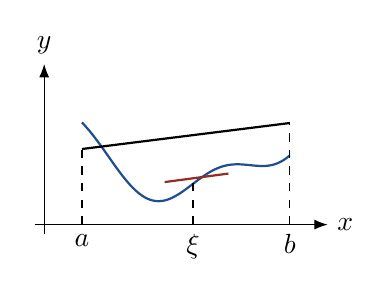
\begin{tikzpicture}[scale=0.60,>=Latex]
  \draw[->] (-0.2,0) -- (6.0,0) node[right] {$x$};
  \draw[->] (0,-0.2) -- (0,3.4) node[above] {$y$};
  \draw[thick,MainBlue,domain=0.8:5.2,smooth,samples=120]
    plot(\x,{0.22*(\x-3)^2+0.75+0.35*sin(120*\x)});
  \draw[thick] (0.8,1.6) -- (5.2,2.15);
  \draw[dashed] (0.8,0) node[below] {$a$} -- (0.8,1.6);
  \draw[dashed] (5.2,0) node[below] {$b$} -- (5.2,2.15);
  \draw[dashed] (3.15,0) node[below] {$\xi$} -- (3.15,0.95);
  \draw[thick,AccentRed] (2.55,0.90) -- (3.90,1.08);
\end{tikzpicture}
\end{center}
\vspace{-0.7em}
\begin{alertblock}{物理含义}
质点的平均速度等于某一点的瞬时速度。
\end{alertblock}
\end{frame}

\begin{frame}{Lagrange 定理的面积证明}
\footnotesize
在曲线上取动点 $(x,f(x))$，考虑三点
\[
  (a,f(a)),\qquad (b,f(b)),\qquad (x,f(x))
\]
所成三角形的有向面积。可用行列式表示为
\[
  \Delta(x)=
  \begin{vmatrix}
  1&1&1\\
  a&b&x\\
  f(a)&f(b)&f(x)
  \end{vmatrix}.
\]
由于 $\Delta(a)=\Delta(b)=0$，由 Rolle 定理，存在 $\xi\in(a,b)$，
使得 $\Delta'(\xi)=0$。

计算导数：
\[
  \Delta'(x)=
  \begin{vmatrix}
  1&1&0\\
  a&b&1\\
  f(a)&f(b)&f'(x)
  \end{vmatrix}
  =(b-a)f'(x)-\bigl(f(b)-f(a)\bigr).
\]
令 $x=\xi$，即得到
\[
  f'(\xi)=\frac{f(b)-f(a)}{b-a}.
\]
\end{frame}

\begin{frame}{Lagrange 定理的常用形式}
\small
\begin{block}{增量公式}
Lagrange 中值定理常写成
\[
  f(b)=f(a)+f'(\xi)(b-a),\qquad a<\xi<b.
\]
若令
\[
  \xi=a+\theta(b-a),\qquad 0<\theta<1,
\]
则
\[
  f(b)=f(a)+f'\bigl(a+\theta(b-a)\bigr)(b-a).
\]
\end{block}

\begin{alertblock}{局部增量写法}
令 $b=x_0+\Delta x,\ a=x_0$，可得
\[
  \Delta y=f'(x_0+\theta\Delta x)\Delta x,\qquad 0<\theta<1.
\]
这就是后面 Taylor 展开的入口。
\end{alertblock}
\end{frame}

\begin{frame}{定理 2.3：Cauchy 中值定理}
\small
\begin{block}{结论}
设 $f,g$ 在 $[a,b]$ 上连续，在 $(a,b)$ 中可微，且
\[
  g'(x)\ne0,\qquad x\in(a,b).
\]
则存在 $\xi\in(a,b)$，使得
\[
  \frac{f(b)-f(a)}{g(b)-g(a)}
  =
  \frac{f'(\xi)}{g'(\xi)}.
\]
\end{block}
\begin{block}{证明思路}
由 Rolle 定理和 $g'\ne0$ 知 $g(b)\ne g(a)$。令
\[
  F(x)=f(x)-\left[f(a)+
  \frac{f(b)-f(a)}{g(b)-g(a)}(g(x)-g(a))\right].
\]
则 $F(a)=F(b)=0$，对 $F$ 使用 Rolle 定理即可。
\end{block}
\end{frame}

\begin{frame}{Cauchy 定理的地位}
\small
\begin{block}{包含 Lagrange 定理}
令 $g(x)=x$，则 $g'(x)=1$，Cauchy 定理变成
\[
  \frac{f(b)-f(a)}{b-a}=f'(\xi),
\]
即 Lagrange 中值定理。
\end{block}
\begin{alertblock}{统一视角}
这些结果都刻画了函数值差与导数值之间的紧密联系。
Newton--Leibniz 公式也是这种联系的一个精确体现。
\end{alertblock}
\end{frame}

\begin{frame}{Cauchy 定理的参数曲线解释}
\small
\begin{block}{把两个函数看成一条曲线}
令
\[
  X=g(t),\qquad Y=f(t),\qquad t\in[a,b].
\]
则端点连线的斜率为
\[
  \frac{f(b)-f(a)}{g(b)-g(a)}.
\]
曲线在参数 $t=\xi$ 处的切线斜率为
\[
  \frac{\dd Y/\dd t}{\dd X/\dd t}
  =
  \frac{f'(\xi)}{g'(\xi)}.
\]
\end{block}

\begin{alertblock}{几何含义}
Cauchy 中值定理说明：在某个参数值 $\xi$ 处，曲线的切线与连接两端点的弦平行。
\end{alertblock}
\end{frame}

\begin{frame}{例 2.1：题目}
\small
\begin{block}{题目}
证明
\[
  |\sin x-\sin y|\le |x-y|,\qquad x,y\in\R.
\]
\end{block}
\end{frame}

\begin{frame}{例 2.1：证明}
\small
若 $x\ne y$，由 Lagrange 中值定理，存在 $\xi$ 介于 $x,y$ 之间，使得
\[
  \sin x-\sin y=\cos \xi\,(x-y).
\]
于是
\[
  |\sin x-\sin y|=|\cos\xi|\,|x-y|\le |x-y|.
\]
当 $x=y$ 时结论显然成立。
\end{frame}

\begin{frame}{例 2.2：题目}
\small
\begin{block}{题目}
设 $f$ 在 $[a,b]$ 上连续，在 $(a,b)$ 中可导，且
\[
  f(a)=f(b)=0.
\]
证明存在 $\xi\in(a,b)$，使得
\[
  f'(\xi)+f(\xi)=0.
\]
\end{block}
\end{frame}

\begin{frame}{例 2.2：证明}
\small
考虑
\[
  g(x)=\ee^x f(x).
\]
则 $g(a)=g(b)=0$，因此可对 $g$ 使用 Rolle 定理。
由 Rolle 定理，存在 $\xi\in(a,b)$，使得
\[
  g'(\xi)=0.
\]
又
\[
  g'(x)=\ee^x f(x)+\ee^x f'(x)
       =\ee^x\bigl(f(x)+f'(x)\bigr).
\]
由于 $\ee^\xi>0$，故
\[
  f'(\xi)+f(\xi)=0.
\]
\end{frame}

\begin{frame}{例 2.3：题目}
\small
\begin{block}{题目}
证明
\[
  \ee^x\ge1+x,\qquad x\in\R,
\]
且等号仅在 $x=0$ 处成立。
\end{block}
\end{frame}

\begin{frame}{例 2.3：证明}
\small
令 $f(x)=\ee^x-(1+x)$，则 $f(0)=0$。
当 $x\ne0$ 时，由 Cauchy 中值定理，可写成 $\xi=\theta x$，
$0<\theta<1$，且
\[
  f(x)=f(x)-f(0)=f'(\xi)x=(\ee^{\theta x}-1)x.
\]
若 $x>0$，则 $\ee^{\theta x}>1$；若 $x<0$，则 $\ee^{\theta x}<1$。
两种情形下均有 $f(x)>0$。
\end{frame}

\begin{frame}{例 2.4：题目}
\small
\begin{block}{题目}
设 $f$ 在 $[a,b]$ 上连续，在 $(a,b)$ 中二阶可导。
如果 $f(a)=f(b)=0$，则对任意 $c\in[a,b]$，存在 $\xi\in(a,b)$，
使得
\[
  f(c)=\frac{f''(\xi)}2(c-a)(c-b).
\]
\end{block}
\end{frame}

\begin{frame}{例 2.4：证明}
\small
不妨设 $c\in(a,b)$。令
\[
  F(x)=f(x)-\frac{f(c)}{(c-a)(c-b)}(x-a)(x-b),
  \qquad x\in[a,b].
\]
则
\[
  F(a)=F(c)=F(b)=0.
\]
由 Rolle 定理，存在
\[
  \xi_1\in(a,c),\qquad \xi_2\in(c,b),
\]
使得
\[
  F'(\xi_1)=0,\qquad F'(\xi_2)=0.
\]
再对 $F'$ 使用 Rolle 定理，存在 $\xi\in(\xi_1,\xi_2)$，使
\[
  F''(\xi)=0.
\]
而
\[
  F''(x)=f''(x)-\frac{2f(c)}{(c-a)(c-b)}.
\]
代入 $x=\xi$，即得
\[
  f(c)=\frac{f''(\xi)}2(c-a)(c-b).
\]
\end{frame}

\begin{frame}{插值余项的一般形式}
\footnotesize
上例可以推广。若 $f$ 是 $n$ 阶可导函数，且 $f(x)=0$ 有 $n$ 个不同解
$x_1,\ldots,x_n$，则对任意 $c\in[a,b]$，存在 $\xi\in(a,b)$，使得
\[
  f(c)=\frac1{n!}f^{(n)}(\xi)\prod_{i=1}^{n}(c-x_i).
\tag{2.1}
\]
证明仍然是构造辅助函数并反复使用 Rolle 定理。

若 $x_1,\ldots,x_n$ 为插值节点，令
\[
  p_{n-1}(x)=
  \sum_{i=1}^{n}\left[
  \prod_{j\ne i}\frac{x-x_j}{x_i-x_j}
  \right]f(x_i),
\]
则
\[
  f(x)-p_{n-1}(x)
  =\frac1{n!}f^{(n)}(\xi)\prod_{i=1}^{n}(x-x_i).
\tag{2.2}
\]
\end{frame}

\begin{frame}{例 2.5：题目}
\small
\begin{block}{题目}
证明勒让德多项式
\[
  \frac{\dd^n}{\dd x^n}(x^2-1)^n
\]
在 $(-1,1)$ 中有 $n$ 个不同实根。
\end{block}
\end{frame}

\begin{frame}{例 2.5：证明}
\small
多项式 $(x^2-1)^n$ 在 $x=-1,1$ 处各有 $n$ 重零点。
由 Rolle 定理，导函数在 $(-1,1)$ 内至少产生一个零点。
反复使用 Rolle 定理，每求一次导数，端点重数下降，并在内部保留足够多零点。

重复这个过程可知，
\[
  \frac{\dd^k}{\dd x^k}(x^2-1)^n
\]
在 $(-1,1)$ 中至少有 $k$ 个不同实根。
取 $k=n$，即得结论。
\end{frame}

\begin{frame}{习题 2.1：题目}
\small
证明多项式
\[
  p(x)=x^3-3x+c
\]
在 $[0,1]$ 上不存在两个不同的实根。
\end{frame}

\begin{frame}{习题 2.1：答案}
\small
若 $p$ 在 $[0,1]$ 上有两个不同实根，则由 Rolle 定理，
存在 $\xi\in(0,1)$ 使得
\[
  p'(\xi)=0.
\]
但
\[
  p'(x)=3x^2-3=3(x^2-1)<0,\qquad x\in(0,1).
\]
矛盾。因此 $p$ 在 $[0,1]$ 上不可能有两个不同实根。
\end{frame}

\begin{frame}{习题 2.2：题目}
\small
设 $f$ 在 $[a,b]$ 上连续，在 $(a,b)$ 中可微，且
\[
  f(a)=f(b)=0.
\]
证明存在 $\xi\in(a,b)$，使得
\[
  f'(\xi)=2f(\xi).
\]
\end{frame}

\begin{frame}{习题 2.2：答案}
\small
令
\[
  g(x)=\ee^{-2x}f(x).
\]
则 $g$ 在 $[a,b]$ 上连续、在 $(a,b)$ 中可微，且 $g(a)=g(b)=0$。
由 Rolle 定理，存在 $\xi\in(a,b)$，使得 $g'(\xi)=0$。

又
\[
  g'(x)=\ee^{-2x}\bigl(f'(x)-2f(x)\bigr),
\]
故
\[
  f'(\xi)=2f(\xi).
\]
\end{frame}

\begin{frame}{习题 2.3：题目}
\small
设 $f$ 在 $[a,b]$ 上二阶可微，且
\[
  f(a)=f(b)=0,\qquad f'_+(a)f'_-(b)>0.
\]
证明存在 $\xi\in(a,b)$，使得
\[
  f''(\xi)=0.
\]
\end{frame}

\begin{frame}{习题 2.3：答案}
\small
若 $f'_+(a)$ 与 $f'_-(b)$ 同为正，则 $f$ 在 $a$ 右侧先为正，
在 $b$ 左侧为负；同为负时方向相反。两种情形下，由连续性可知，
存在 $c\in(a,b)$，使
\[
  f(c)=0.
\]
于是 $f(a)=f(c)=f(b)=0$。
对 $[a,c]$ 与 $[c,b]$ 分别用 Rolle 定理，得到
\[
  f'(\eta_1)=f'(\eta_2)=0,\qquad \eta_1\in(a,c),\ \eta_2\in(c,b).
\]
再对 $f'$ 在 $[\eta_1,\eta_2]$ 上用 Rolle 定理，得到某个
$\xi\in(\eta_1,\eta_2)$ 满足 $f''(\xi)=0$。
\end{frame}

\begin{frame}{习题 2.4：题目}
\small
证明
\[
  \ee^x>1+x+\frac{x^2}{2!}+\frac{x^3}{3!},
  \qquad x\ne0.
\]
\end{frame}

\begin{frame}{习题 2.4：答案}
\small
令
\[
  F(x)=\ee^x-1-x-\frac{x^2}{2}-\frac{x^3}{6}.
\]
则
\[
  F(0)=F'(0)=F''(0)=0,\qquad F'''(x)=\ee^x-1.
\]
若 $x>0$，则 $F'''(x)>0$，从而 $F''$、$F'$、$F$ 从 $0$ 起依次严格增加，
所以 $F(x)>0$。

若 $x<0$，在区间 $(x,0)$ 上 $F'''<0$，可反向推出
\[
  F''(x)>0,\qquad F'(x)<0,\qquad F(x)>0.
\]
故原不等式对 $x\ne0$ 成立。
\end{frame}

\begin{frame}{习题 2.5：题目}
\small
设 $f$ 在 $[a,b]$ 上连续，在 $(a,b)$ 中二阶可导。
若 $l$ 是满足
\[
  l(a)=f(a),\qquad l(b)=f(b)
\]
的线性函数，证明对任意 $c\in[a,b]$，存在 $\xi\in(a,b)$，使得
\[
  f(c)-l(c)=\frac{f''(\xi)}2(c-a)(c-b).
\]
\end{frame}

\begin{frame}{习题 2.5：答案}
\small
令
\[
  h(x)=f(x)-l(x).
\]
则 $h(a)=h(b)=0$，且 $h''(x)=f''(x)$。
对 $h$ 使用例 2.4 的二阶余项公式，得存在 $\xi\in(a,b)$，使
\[
  h(c)=\frac{h''(\xi)}2(c-a)(c-b).
\]
代回 $h=f-l$，即
\[
  f(c)-l(c)=\frac{f''(\xi)}2(c-a)(c-b).
\]
\end{frame}

\begin{frame}{习题 2.6：题目}
\small
设 $f$ 为 $[a,b]$ 上的三阶可导函数，且
\[
  f(a)=f'(a)=f(b)=0.
\]
证明任给 $c\in[a,b]$，存在 $\xi\in(a,b)$，使
\[
  f(c)=\frac16 f^{(3)}(\xi)(c-a)^2(c-b).
\]
\end{frame}

\begin{frame}{习题 2.6：答案}
\footnotesize
当 $c=a$ 或 $c=b$ 时结论显然。设 $c\in(a,b)$，令
\[
  F(x)=f(x)-\frac{f(c)}{(c-a)^2(c-b)}(x-a)^2(x-b).
\]
则
\[
  F(a)=F'(a)=F(c)=F(b)=0.
\]
由 Rolle 定理，$F'$ 在 $(a,c)$ 与 $(c,b)$ 中分别有零点
$\eta_1,\eta_2$；同时 $F'(a)=0$。
再对 $F'$ 两次使用 Rolle 定理，可得某个 $\xi\in(a,b)$ 使
\[
  F^{(3)}(\xi)=0.
\]
又
\[
  F^{(3)}(x)=f^{(3)}(x)-6\frac{f(c)}{(c-a)^2(c-b)},
\]
故
\[
  f(c)=\frac16 f^{(3)}(\xi)(c-a)^2(c-b).
\]
\end{frame}

\begin{frame}{习题 2.7：题目}
\small
证明多项式
\[
  \ee^x\frac{\dd^n}{\dd x^n}(x^n\ee^{-x})
\]
有 $n$ 个正的实根。
\end{frame}

\begin{frame}{习题 2.7：答案}
\small
令
\[
  u(x)=x^n\ee^{-x}.
\]
乘以 $\ee^x>0$ 不改变零点，因此只需证明 $u^{(n)}$ 有 $n$ 个正根。

$u$ 在 $x=0$ 处有 $n$ 重零点，且 $u(x)\to0$ $(x\to+\infty)$。
对 $u$ 在 $(0,+\infty)$ 上反复使用 Rolle 定理：每求一次导数，
原点处零点重数减少 $1$，同时在正半轴上新增一个零点。
归纳可知，$u^{(k)}$ 在 $(0,+\infty)$ 中至少有 $k$ 个不同零点。
取 $k=n$ 即得结论。
\end{frame}

\begin{frame}{习题 2.8：题目}
\small
设函数 $f$ 在区间 $[a,b]$ 上可导，且存在 $M>0$，使得
\[
  |f'(x)|\le M,\qquad x\in[a,b].
\]
证明
\[
  \left|f(x)-\frac{f(a)+f(b)}2\right|
  \le\frac12M(b-a),\qquad x\in[a,b].
\]
\end{frame}

\begin{frame}{习题 2.8：答案}
\small
由 Lagrange 中值定理，
\[
  |f(x)-f(a)|\le M(x-a),\qquad
  |f(b)-f(x)|\le M(b-x).
\]
于是
\[
\begin{aligned}
\left|f(x)-\frac{f(a)+f(b)}2\right|
&=\frac12\left|(f(x)-f(a))+(f(x)-f(b))\right|\\
&\le \frac12\bigl(|f(x)-f(a)|+|f(x)-f(b)|\bigr)\\
&\le\frac12M(b-a).
\end{aligned}
\]
\end{frame}

\begin{frame}{习题 2.9：题目}
\small
设函数 $f$ 在点 $x_0$ 处可导，$x_n<x_0<y_n$，且
\[
  x_n\to x_0,\qquad y_n\to x_0.
\]
证明
\[
  \lim_{n\to\infty}\frac{f(x_n)-f(y_n)}{x_n-y_n}=f'(x_0).
\]
\end{frame}

\begin{frame}{习题 2.9：答案}
\small
令
\[
  A_n=\frac{f(x_n)-f(x_0)}{x_n-x_0},\qquad
  B_n=\frac{f(y_n)-f(x_0)}{y_n-x_0}.
\]
由 $f$ 在 $x_0$ 处可导，$A_n\to f'(x_0)$，$B_n\to f'(x_0)$。

设 $\alpha_n=x_0-x_n>0$，$\beta_n=y_n-x_0>0$。则
\[
  \frac{f(x_n)-f(y_n)}{x_n-y_n}
  =
  \frac{\alpha_n A_n+\beta_n B_n}{\alpha_n+\beta_n}.
\]
右侧是 $A_n,B_n$ 的加权平均，因此极限为 $f'(x_0)$。
\end{frame}

\begin{frame}{习题 2.10：题目}
\small
设函数 $f$ 在 $(a,b)$ 中可微，且
\[
  a<x_i\le y_i<b,\qquad i=1,2,\ldots,n.
\]
证明存在 $\xi\in(a,b)$，使得
\[
  \sum_{i=1}^n\bigl[f(y_i)-f(x_i)\bigr]
  =f'(\xi)\sum_{i=1}^n(y_i-x_i).
\]
\end{frame}

\begin{frame}{习题 2.10：答案}
\footnotesize
若某些 $x_i=y_i$，其项为零，可删去。设
\[
  S=\sum_{i=1}^n(y_i-x_i)>0.
\]
对每个 $[x_i,y_i]$ 用 Lagrange 定理，存在 $\eta_i\in(x_i,y_i)$，使
\[
  f(y_i)-f(x_i)=f'(\eta_i)(y_i-x_i).
\]
因此
\[
  A=\frac{\sum_{i=1}^n[f(y_i)-f(x_i)]}{S}
\]
是若干个 $f'(\eta_i)$ 的加权平均，故介于这些值的最小值和最大值之间。
导函数 $f'$ 具有 Darboux 性质，所以存在 $\xi\in(a,b)$，使
$f'(\xi)=A$。整理即得结论。
\end{frame}

\begin{frame}{习题 2.11：题目}
\small
设 $f$ 在 $[a,+\infty)$ 中可微，且
\[
  f(a)=0,\qquad |f'(x)|\le |f(x)|,\quad x\in[a,+\infty).
\]
证明
\[
  f\equiv0.
\]
\end{frame}

\begin{frame}{习题 2.11：答案}
\small
先在任意长度小于 $1$ 的区间 $[a,a+h]$ 上证明。
设
\[
  M_h=\max_{[a,a+h]}|f(x)|.
\]
若最大值在 $c$ 处取得，则由 Lagrange 中值定理，
\[
  |f(c)|=|f(c)-f(a)|\le \max_{[a,a+h]}|f'(x)|\,h
  \le M_h h.
\]
当 $0<h<1$ 时，只能有 $M_h=0$，故 $f\equiv0$ 于 $[a,a+h]$。

再从 $a+h$ 开始重复上述论证，逐段推进，可得
$f\equiv0$ 于整个 $[a,+\infty)$。
\end{frame}

\begin{frame}{§2 提高题：从中值定理到导函数性质}
\small
下面几题把本节的核心方法继续推进：
\[
  \text{构造辅助函数}
  \quad+\quad
  \text{中值定理}
  \quad+\quad
  \text{导函数的介值性}.
\]

\begin{block}{学习目标}
不仅会套用 Rolle、Lagrange、Cauchy 定理，还要学会判断：
\begin{itemize}
  \item 什么时候应构造原函数或辅助函数；
  \item 什么时候应把差商改写成导数；
  \item 导函数为什么不能像普通函数那样跳跃。
\end{itemize}
\end{block}
\end{frame}

\begin{frame}{习题 2.12：题目}
\small
设
\[
  \frac{a_0}{n+1}+\frac{a_1}{n}+\cdots+a_n=0.
\]
证明方程
\[
  a_0x^n+a_1x^{n-1}+\cdots+a_n=0
\]
在区间 $(0,1)$ 中至少有一个根。
\end{frame}

\begin{frame}{习题 2.12：答案}
\small
构造辅助函数
\[
  F(x)=\frac{a_0}{n+1}x^{n+1}
       +\frac{a_1}{n}x^n+\cdots+a_nx.
\]
则
\[
  F(0)=0,\qquad
  F(1)=\frac{a_0}{n+1}+\frac{a_1}{n}+\cdots+a_n=0.
\]
由 Rolle 定理，存在 $\xi\in(0,1)$，使
\[
  F'(\xi)=0.
\]
而
\[
  F'(x)=a_0x^n+a_1x^{n-1}+\cdots+a_n,
\]
故原方程在 $(0,1)$ 中至少有一个根。
\end{frame}

\begin{frame}{习题 2.13：题目}
\small
设 $f$ 在 $[a,a+\delta]$ 上连续，在 $(a,a+\delta)$ 中可导，且
\[
  \lim_{x\to a+}f'(x)=A
\]
存在。证明 $f$ 在 $a$ 处存在右导数，且
\[
  f'_+(a)=A.
\]
\end{frame}

\begin{frame}{习题 2.13：答案}
\small
对任意足够小的 $h>0$，在 $[a,a+h]$ 上使用 Lagrange 中值定理，
存在 $\theta_h\in(0,1)$，使得
\[
  \frac{f(a+h)-f(a)}{h}=f'(a+\theta_hh).
\]
由于
\[
  a+\theta_hh\to a+ \qquad (h\to0+),
\]
由题设得
\[
  f'(a+\theta_hh)\to A.
\]
因此
\[
  f'_+(a)=
  \lim_{h\to0+}\frac{f(a+h)-f(a)}h=A.
\]
\end{frame}

\begin{frame}{习题 2.14：题目}
\small
设 $f$ 在区间 $I$ 上可导。证明：导函数 $f'$ 不可能有第一类间断点。
\end{frame}

\begin{frame}{习题 2.14：答案}
\small
反设 $f'$ 在某个内点 $c$ 有第一类间断点。则 $f'(c-)$ 与 $f'(c+)$
作为有限单侧极限存在，但不能同时等于 $f'(c)$。

由习题 2.13 的右侧版本，
\[
  f'_+(c)=f'(c+).
\]
同理，由左侧版本，
\[
  f'_-(c)=f'(c-).
\]
但 $f$ 在 $c$ 处可导，所以
\[
  f'_-(c)=f'(c)=f'_+(c).
\]
于是
\[
  f'(c-)=f'(c)=f'(c+),
\]
这说明 $f'$ 在 $c$ 处并非第一类间断点，矛盾。
\end{frame}

\begin{frame}{习题 2.15：题目}
\small
设 $I$ 为区间，$f$ 在 $I$ 中可微。若存在常数 $L>0$，使得对 $I$
中所有内点 $x$ 都有
\[
  |f'(x)|\le L,
\]
证明 $f$ 在区间 $I$ 上满足 Lipschitz 条件：
\[
  |f(x_1)-f(x_2)|\le L|x_1-x_2|.
\]
\end{frame}

\begin{frame}{习题 2.15：答案}
\small
任取 $x_1,x_2\in I$，不妨设 $x_1<x_2$。
由 Lagrange 中值定理，存在 $\xi\in(x_1,x_2)$，使得
\[
  f(x_2)-f(x_1)=f'(\xi)(x_2-x_1).
\]
取绝对值，得
\[
  |f(x_2)-f(x_1)|
  =
  |f'(\xi)|\,|x_2-x_1|
  \le L|x_2-x_1|.
\]
这正是 Lipschitz 条件。
\end{frame}

\begin{frame}{习题 2.16：题目}
\small
设 $f\in C[0,1]$，在 $(0,1)$ 中可微，且
\[
  f(0)=0,\qquad f(1)=1.
\]
又设 $k_1,\ldots,k_n$ 为满足
\[
  k_1+\cdots+k_n=1
\]
的正数。证明：在 $(0,1)$ 中存在 $n$ 个互不相同的数
$t_1,\ldots,t_n$，使得
\[
  \frac{k_1}{f'(t_1)}+\frac{k_2}{f'(t_2)}+\cdots+\frac{k_n}{f'(t_n)}=1.
\]
\end{frame}

\begin{frame}{习题 2.16：答案}
\footnotesize
设
\[
  s_i=k_1+\cdots+k_i,\qquad i=1,\ldots,n.
\]
由连续性和介值定理，可递归地在 $[x_{i-1},1]$ 中选取 $x_i$，得到
\[
  0=x_0<x_1<\cdots<x_{n-1}<x_n=1
\]
使得
\[
  f(x_i)=s_i,\qquad i=1,\ldots,n.
\]
在每个区间 $[x_{i-1},x_i]$ 上用 Lagrange 中值定理，存在
$t_i\in(x_{i-1},x_i)$，使
\[
  k_i=f(x_i)-f(x_{i-1})=f'(t_i)(x_i-x_{i-1}).
\]
因此
\[
  \frac{k_i}{f'(t_i)}=x_i-x_{i-1}.
\]
求和得
\[
  \sum_{i=1}^n\frac{k_i}{f'(t_i)}
  =
  \sum_{i=1}^n(x_i-x_{i-1})=1.
\]
\end{frame}

\begin{frame}{习题 2.17：题目}
\small
设 $f$ 在点 $a$ 处二阶可导，且
\[
  f''(a)\ne0.
\]
当 $h$ 充分小时，由 Lagrange 中值定理可写成
\[
  f(a+h)-f(a)=f'(a+\theta(h)h)h,\qquad 0<\theta(h)<1.
\]
证明
\[
  \lim_{h\to0}\theta(h)=\frac12.
\]
\end{frame}

\begin{frame}{习题 2.17：答案}
\small
由二阶可导性，
\[
  f(a+h)-f(a)
  =
  f'(a)h+\frac12f''(a)h^2+o(h^2).
\]
另一方面，
\[
  f'(a+\theta h)
  =
  f'(a)+f''(a)\theta h+o(h),
\]
其中 $0<\theta<1$，所以 $\theta h\to0$。代入中值公式，
\[
  f(a+h)-f(a)=
  \bigl(f'(a)+f''(a)\theta h+o(h)\bigr)h.
\]
比较 $h^2$ 项：
\[
  \frac12f''(a)+o(1)=\theta(h)f''(a)+o(1).
\]
因 $f''(a)\ne0$，故
\[
  \theta(h)\to\frac12.
\]
\end{frame}

\begin{frame}{习题 2.18：题目}
\small
设 $I$ 为区间，$f,g\in C(I)$。若除有限个点外，在区间 $I$ 中都有
\[
  f'(x)=g'(x),
\]
证明存在常数 $C$，使得在整个区间 $I$ 上
\[
  f(x)=g(x)+C.
\]
\end{frame}

\begin{frame}{习题 2.18：答案}
\small
令
\[
  F(x)=f(x)-g(x).
\]
在除去有限个例外点后，区间 $I$ 被分成有限个小区间。
在每个小区间内，
\[
  F'(x)=f'(x)-g'(x)=0.
\]
由“导数恒为零则函数为常数”，$F$ 在每个小区间上都是常数。

由于 $F=f-g$ 在 $I$ 上连续，相邻小区间在公共端点处的常数值必须相等。
因此 $F$ 在整个 $I$ 上为同一个常数 $C$，即
\[
  f(x)=g(x)+C.
\]
\end{frame}

\section{单调函数}

\begin{frame}{§3 单调函数}
\small
\begin{block}{问题}
微分中值定理可以把导数信息转化为函数值信息。
因此，若能控制 $f'$ 的符号，就能控制 $f$ 的单调性和极值。
\end{block}
\begin{alertblock}{常用模板}
取 $x_1<x_2$，由 Lagrange 中值定理，
\[
  f(x_2)-f(x_1)=f'(\xi)(x_2-x_1).
\]
由于 $x_2-x_1>0$，差值符号由 $f'(\xi)$ 的符号控制。
\end{alertblock}
\end{frame}

\begin{frame}{命题 3.1：导数恒为零}
\small
\begin{block}{结论}
设 $f$ 在 $[a,b]$ 上连续，在 $(a,b)$ 中可微。
如果
\[
  f'(x)=0,\qquad x\in(a,b),
\]
则 $f$ 为常值函数。
\end{block}
\begin{block}{证明}
任取 $x,y\in[a,b]$。由 Lagrange 中值定理，存在 $\xi$ 介于 $x,y$ 之间，
使得
\[
  f(x)-f(y)=f'(\xi)(x-y)=0.
\]
因此 $f(x)=f(y)$。
\end{block}
\end{frame}

\begin{frame}{命题 3.2：单调性的导数判别}
\small
\begin{block}{结论}
设 $f$ 在 $[a,b]$ 上连续，在 $(a,b)$ 中可微。则
\[
  f\text{ 为单调函数}
  \quad\Longleftrightarrow\quad
  f'\text{ 不变号}.
\]
\end{block}
\begin{block}{证明方向一}
若 $f$ 单调递增，则对 $x_0\in(a,b)$，
\[
  f'(x_0)=\lim_{x\to x_0}
  \frac{f(x)-f(x_0)}{x-x_0}\ge0.
\]
单调递减同理得到 $f'(x_0)\le0$。
\end{block}
\end{frame}

\begin{frame}{命题 3.2：充分性}
\small
\begin{block}{证明方向二}
若 $f'(x)\ge0$，任取 $x_1<x_2$。由 Lagrange 中值定理，
存在 $\xi\in(x_1,x_2)$，使得
\[
  f(x_2)-f(x_1)=f'(\xi)(x_2-x_1)\ge0.
\]
故 $f$ 单调递增。$f'\le0$ 时同理。
\end{block}
\begin{alertblock}{注意}
如果 $f'>0$，则 $f$ 严格单调递增；如果 $f'<0$，则 $f$ 严格单调递减。
反之不然，例如 $f(x)=x^3$ 严格单调递增，但 $f'(0)=0$。
\end{alertblock}
\end{frame}

\begin{frame}{两个驻点之间的单调性}
\small
如果可微函数在两个驻点之间没有其他驻点，则导数在这两个驻点之间不变号。
因此函数图像在这段区间中大体保持单调方向。

\begin{block}{理由}
若 $f'$ 在两个点之间改变符号，由 Darboux 定理，$f'$ 会取到 $0$。
这会产生新的驻点，与假设矛盾。
\end{block}
\end{frame}

\begin{frame}{定理 3.3：反函数定理}
\small
\begin{block}{结论}
设 $f$ 为区间 $I$ 中的可微函数。如果 $f'$ 处处非零，
则 $f^{-1}$ 是可导的，且其逆函数也可微。
\end{block}
\begin{block}{证明思路}
若 $f'(x)\ne0$，由 Darboux 定理可知 $f'$ 不能从正值跳到负值，
因此 $f'$ 不变号。由单调性判别，$f$ 单射，从而 $f^{-1}$ 存在。
再由反函数求导公式，
\[
  (f^{-1})'(y)=\frac1{f'(x)},\qquad y=f(x),
\]
得到 $f^{-1}$ 可微。
\end{block}
\end{frame}

\begin{frame}{命题 3.4：一阶导数判别极值}
\small
\begin{block}{结论}
设 $\delta>0$，$f$ 在 $(x_0-\delta,x_0+\delta)$ 中连续，
在去心邻域中可微。

若
\[
  f'(x)\le0,\quad x\in(x_0-\delta,x_0),
  \qquad
  f'(x)\ge0,\quad x\in(x_0,x_0+\delta),
\]
则 $x_0$ 为极小值点。

若左侧 $f'\ge0$、右侧 $f'\le0$，则 $x_0$ 为极大值点。
\end{block}
\end{frame}

\begin{frame}{一阶导数判别的证明}
\small
以第一种情形为例。任取 $x\in(x_0-\delta,x_0)$，
由 Lagrange 中值定理，存在 $\xi\in(x,x_0)$，使得
\[
  f(x)-f(x_0)=f'(\xi)(x-x_0).
\]
此时 $f'(\xi)\le0$ 且 $x-x_0<0$，故
\[
  f(x)-f(x_0)\ge0.
\]
任取 $x\in(x_0,x_0+\delta)$，同理
\[
  f(x)-f(x_0)=f'(\xi)(x-x_0)\ge0.
\]
因此 $x_0$ 为极小值点。
\end{frame}

\begin{frame}{例 3.1：题目}
\small
\begin{block}{题目}
设 $x>-1$ 且 $x\ne0$，证明
\[
  \frac{x}{1+x}<\ln(1+x)<x.
\]
\end{block}
\end{frame}

\begin{frame}{例 3.1：证明}
\small
令 $f(x)=\ln(1+x)-x$，则 $f(0)=0$，且
\[
  f'(x)=\frac1{1+x}-1=-\frac{x}{1+x}.
\]
所以 $f$ 在 $(-1,0)$ 上严格递增，在 $(0,+\infty)$ 上严格递减，
从而 $f(x)<f(0)=0$，即 $\ln(1+x)<x$。

再令 $g(x)=\ln(1+x)-\frac{x}{1+x}$，有
\[
  g'(x)=\frac{x}{(1+x)^2}.
\]
同理得到 $g(x)>0$。
\end{frame}

\begin{frame}{例 3.2：题目}
\small
\begin{block}{题目}
设 $b>a>1$，证明
\[
  ba^b>ab^a.
\]
\end{block}
\end{frame}

\begin{frame}{例 3.2：证明}
\small
两边取对数，原不等式等价于
\[
  \ln b+b\ln a>\ln a+a\ln b
  \quad\Longleftrightarrow\quad
  \frac{\ln a}{a-1}>\frac{\ln b}{b-1}.
\]
考虑
\[
  f(x)=\frac{\ln x}{x-1},\qquad x>1.
\]
则
\[
  f'(x)=\frac{(x-1)-x\ln x}{x(x-1)^2}<0,\qquad x>1.
\]
故 $f$ 在 $(1,+\infty)$ 上严格递减，结论成立。
\end{frame}

\begin{frame}{命题 3.5：二阶导数判别}
\small
\begin{block}{结论}
设 $f$ 在 $x_0$ 处二阶可导，且 $f'(x_0)=0$。
\begin{enumerate}
  \item 若 $f''(x_0)>0$，则 $x_0$ 为严格极小值点。
  \item 若 $f''(x_0)<0$，则 $x_0$ 为严格极大值点。
\end{enumerate}
\end{block}
\begin{block}{证明要点}
若 $f''(x_0)>0$，则
\[
  \lim_{x\to x_0}\frac{f'(x)-f'(x_0)}{x-x_0}=f''(x_0)>0.
\]
因此在 $x_0$ 左侧 $f'(x)<0$，右侧 $f'(x)>0$。
由一阶导数判别，$x_0$ 为严格极小值点。
\end{block}
\end{frame}

\begin{frame}{推论 3.6：极值点的必要条件}
\small
\begin{block}{结论}
设 $f$ 在 $x_0$ 处二阶可导。
若 $x_0$ 为 $f$ 的极小值点，则
\[
  f''(x_0)\ge0;
\]
若 $x_0$ 为 $f$ 的极大值点，则
\[
  f''(x_0)\le0.
\]
\end{block}
\begin{alertblock}{注意}
若 $f'(x_0)=0$ 且 $f''(x_0)=0$，则 $x_0$ 可能是极值点，也可能不是。
此时常需用更高阶导数或 Taylor 展开进一步判断。
\end{alertblock}
\end{frame}

\begin{frame}{例 3.3：题目}
\small
\begin{block}{题目}
证明
\[
  \sin x\ge x-\frac{x^3}{6},\qquad x\ge0,
\]
且等号仅当 $x=0$ 时成立。
\end{block}
\end{frame}

\begin{frame}{例 3.3：证明}
\small
令
\[
  f(x)=\sin x-x+\frac{x^3}{6}.
\]
则
\[
  f'(x)=\cos x-1+\frac{x^2}{2},\qquad
  f''(x)=-\sin x+x\ge0,\quad x\ge0.
\]
故 $f'$ 单调递增。又 $f'(0)=0$，所以 $f'(x)\ge0$。
因此 $f$ 在 $[0,+\infty)$ 上单调递增，且 $f(0)=0$，结论成立。
\end{frame}

\begin{frame}{例 3.4：题目}
\small
\begin{block}{题目}
求函数
\[
  f(x)=(x-1)x^{2/3}
\]
的极值。
\end{block}
\end{frame}

\begin{frame}{例 3.4：答案}
\small
当 $x\ne0$ 时，
\[
  f'(x)=x^{2/3}+\frac23(x-1)x^{-1/3}
       =\frac13x^{-1/3}(5x-2).
\]
驻点为
\[
  x=\frac25,
\]
不可导点 $x=0$ 也可能为极值点。

\[
\begin{array}{c|ccc}
x & (-\infty,0) & (0,2/5) & (2/5,+\infty)\\ \hline
f'(x) & + & - & +
\end{array}
\]
因此 $f$ 在 $(-\infty,0)$ 中单调递增，在 $(0,2/5)$ 中单调递减，
在 $(2/5,+\infty)$ 中单调递增。

\[
  x=0 \text{ 为极大值点},\qquad f(0)=0;
\]
\[
  x=\frac25 \text{ 为极小值点},\qquad
  f\left(\frac25\right)
  =-\frac35\sqrt[3]{\frac4{25}}.
\]
\end{frame}

\begin{frame}{习题 3.1：题目}
\small
证明：
\[
  \arcsin x+\arccos x=\frac\pi2,\qquad x\in[-1,1],
\]
\[
  2\arctan x+\arcsin\frac{2x}{1+x^2}=\pi,\qquad x\ge1.
\]
\end{frame}

\begin{frame}{习题 3.1：答案}
\small
令 $F(x)=\arcsin x+\arccos x$。在 $(-1,1)$ 上
\[
  F'(x)=\frac1{\sqrt{1-x^2}}-\frac1{\sqrt{1-x^2}}=0.
\]
故 $F$ 为常数，由 $F(0)=\pi/2$ 得第一式。

令
\[
  G(x)=2\arctan x+\arcsin\frac{2x}{1+x^2}.
\]
当 $x>1$ 时，
\[
  G'(x)=\frac2{1+x^2}-\frac2{1+x^2}=0.
\]
故 $G$ 为常数。由 $G(1)=\pi/2+\pi/2=\pi$，得第二式。
\end{frame}

\begin{frame}{习题 3.2：题目}
\footnotesize
证明下列不等式：
\[
  \tan x>x+\frac{x^3}{3},\qquad x\in\left(0,\frac\pi2\right);
\]
\[
  \frac{2x}{\pi}<\sin x<x,\qquad x\in\left(0,\frac\pi2\right);
\]
\[
  x-\frac{x^2}{2}<\ln(1+x)<x-\frac{x^2}{2(1+x)},\qquad x>-1;
\]
\[
  ny^{n-1}(x-y)<x^n-y^n<nx^{n-1}(x-y),
  \quad n>1,\ x>y.
\]
\end{frame}

\begin{frame}{习题 3.2：答案}
\scriptsize
\begin{enumerate}
  \item 令 $F=\tan x-x-x^3/3$。因 $\tan x>x$，
  \[
    F'(x)=\tan^2x-x^2>0,\quad F(0)=0,
  \]
  故 $F(x)>0$。
  \item $\sin x<x$ 由 $x-\sin x$ 单调递增得出；
  $\sin x>2x/\pi$ 由 $\sin x$ 在 $[0,\pi/2]$ 上为凹函数、图像在弦上方得出。
  \item 原式在 $x>0$ 时成立。令
  \[
    A=\ln(1+x)-x+\frac{x^2}{2},\qquad
    B=\ln(1+x)-x+\frac{x^2}{2(1+x)}.
  \]
  则
  \[
    A'=\frac{x^2}{1+x}>0,\qquad
    B'=-\frac{x^2}{2(1+x)^2}<0.
  \]
  因 $A(0)=B(0)=0$，故 $x>0$ 时 $A>0>B$。若 $-1<x<0$，两边不等号方向相反。
  \item 此式通常需 $x>y>0$。由 Lagrange 定理，
  \[
    x^n-y^n=n\xi^{\,n-1}(x-y),\qquad y<\xi<x.
  \]
  因 $t^{n-1}$ 在正半轴递增，故结论成立。
\end{enumerate}
\end{frame}

\begin{frame}{习题 3.3：题目}
\small
证明
\[
  \ee^x>1+x+\frac{x^2}{2!}+\cdots+\frac{x^n}{n!},
  \qquad x>0.
\]
\end{frame}

\begin{frame}{习题 3.3：答案}
\small
令
\[
  F(x)=\ee^x-\sum_{k=0}^{n}\frac{x^k}{k!}.
\]
则
\[
  F(0)=F'(0)=\cdots=F^{(n)}(0)=0,\qquad
  F^{(n+1)}(x)=\ee^x>0.
\]
从 $F^{(n)}$ 开始向下逐次积分式地理解单调性：
在 $x>0$ 上，$F^{(n)}$ 严格递增且 $F^{(n)}(0)=0$，故 $F^{(n)}>0$；
进而 $F^{(n-1)}>0,\ldots,F>0$。
因此原不等式成立。
\end{frame}

\begin{frame}{习题 3.4：题目}
\small
证明
\[
  \frac{\tan x}{x}>\frac{x}{\sin x},
  \qquad x\in\left(0,\frac\pi2\right).
\]
\end{frame}

\begin{frame}{习题 3.4：答案}
\small
原式等价于
\[
  \frac{\sin^2 x}{x^2\cos x}>1.
\]
令
\[
  F(x)=2\ln\sin x-2\ln x-\ln\cos x.
\]
则
\[
  F'(x)=2\cot x-\frac2x+\tan x.
\]
将分母通分得，$F'(x)>0$ 等价于
\[
  x(1+\cos^2x)>\sin2x.
\]
而 $\sin2x=2\sin x\cos x<2x\cos x\le x(1+\cos^2x)$。
故 $F'(x)>0$，且 $F(0+)=0$，所以 $F(x)>0$，结论成立。
\end{frame}

\begin{frame}{习题 3.5：题目}
\small
证明方程
\[
  x-\frac12\sin x=0
\]
只有唯一的实根。
\end{frame}

\begin{frame}{习题 3.5：答案}
\small
令
\[
  f(x)=x-\frac12\sin x.
\]
则
\[
  f'(x)=1-\frac12\cos x\ge\frac12>0.
\]
因此 $f$ 在 $\R$ 上严格单调递增。
又
\[
  f(0)=0,
\]
所以方程只有唯一实根
\[
  x=0.
\]
\end{frame}

\begin{frame}{习题 3.6：题目}
\small
数列
\[
  1,\ \sqrt2,\ \sqrt[3]{3},\ldots,\sqrt[n]{n},\ldots
\]
中哪一项最大？
\end{frame}

\begin{frame}{习题 3.6：答案}
\small
考虑连续函数
\[
  f(x)=x^{1/x},\qquad x>0.
\]
取对数，令
\[
  g(x)=\ln f(x)=\frac{\ln x}{x}.
\]
则
\[
  g'(x)=\frac{1-\ln x}{x^2}.
\]
所以 $g$ 在 $(0,\ee)$ 上递增，在 $(\ee,+\infty)$ 上递减。
整数项只需比较 $n=2,3$：
\[
  \sqrt2<\sqrt[3]{3}
  \quad\Longleftrightarrow\quad 2^3<3^2.
\]
故最大项为
\[
  \sqrt[3]{3}.
\]
\end{frame}

\begin{frame}{习题 3.7：题目}
\small
研究函数
\[
  \frac{x}{\sin x}
  \quad\text{和}\quad
  \frac{\tan x}{x}
\]
在 $x\in(0,\pi)$ 中的单调性。
\end{frame}

\begin{frame}{习题 3.7：答案}
\footnotesize
对
\[
  F(x)=\frac{x}{\sin x}
\]
有
\[
  F'(x)=\frac{\sin x-x\cos x}{\sin^2x}.
\]
令 $\phi(x)=\sin x-x\cos x$，则
\[
  \phi'(x)=x\sin x>0,\qquad \phi(0+)=0.
\]
故 $F$ 在 $(0,\pi)$ 上严格递增。

对
\[
  G(x)=\frac{\tan x}{x}
\]
有
\[
  G'(x)=\frac{x\sec^2x-\tan x}{x^2}
       =\frac{x-\sin x\cos x}{x^2\cos^2x}.
\]
分子导数为 $2\sin^2x>0$，故分子为正。
因此 $G$ 在 $(0,\pi/2)$ 与 $(\pi/2,\pi)$ 上分别严格递增。
\end{frame}

\begin{frame}{习题 3.8：题目}
\small
研究函数
\[
  \left(1+\frac1x\right)^x,\qquad x>0
\]
的单调性。
\end{frame}

\begin{frame}{习题 3.8：答案}
\small
令
\[
  F(x)=\left(1+\frac1x\right)^x,\qquad
  L(x)=\ln F(x)=x\ln\left(1+\frac1x\right).
\]
则
\[
  L'(x)=\ln\left(1+\frac1x\right)-\frac1{x+1}.
\]
令 $t=1/x>0$，则
\[
  L'(x)=\ln(1+t)-\frac{t}{1+t}.
\]
由例 3.1 的不等式 $\ln(1+t)>t/(1+t)$，得 $L'(x)>0$。
因此 $F$ 在 $(0,+\infty)$ 上严格递增。
\end{frame}

\begin{frame}{习题 3.9：题目}
\small
研究函数
\[
  \frac1{\sin x}-\frac1x,\qquad x\in(0,\pi)
\]
的单调性。
\end{frame}

\begin{frame}{习题 3.9：答案}
\small
令
\[
  F(x)=\frac1{\sin x}-\frac1x.
\]
则
\[
  F'(x)=\frac1{x^2}-\frac{\cos x}{\sin^2x}
       =\frac{\sin^2x-x^2\cos x}{x^2\sin^2x}.
\]
若 $x\in(\pi/2,\pi)$，则 $\cos x<0$，故 $F'(x)>0$。
若 $x\in(0,\pi/2)$，习题 3.4 已证
\[
  \sin^2x>x^2\cos x.
\]
所以 $F'(x)>0$。故 $F$ 在 $(0,\pi)$ 上严格递增。
\end{frame}

\begin{frame}{习题 3.10：题目}
\small
设连续函数 $f(x)$ 在区间 $I$ 中有唯一的极值点。
证明该极值点为最值点。
\end{frame}

\begin{frame}{习题 3.10：答案}
\small
设唯一极值点 $x_0$ 为局部最大值点。若它不是最大值点，
则存在 $y\in I$，使得 $f(y)>f(x_0)$。不妨设 $y>x_0$。

由于 $x_0$ 是局部最大值点，可取 $z\in(x_0,y)$，使
\[
  f(z)<f(x_0)<f(y).
\]
连续函数在 $[x_0,y]$ 上取到最小值。由于区间内已有 $z$ 满足
$f(z)<f(x_0)$，且 $f(y)>f(x_0)$，最小值点既不是 $x_0$ 也不是 $y$，
只能在 $(x_0,y)$ 内部取得，从而给出一个新的局部最小值点，矛盾。

故 $x_0$ 必为最大值点。局部最小值点情形同理。
\end{frame}

\begin{frame}{习题 3.11：题目}
\small
设 $f(x)$ 为 $(-\infty,+\infty)$ 中的有界二次可微函数。
证明存在 $\xi\in\R$，使得
\[
  f''(\xi)=0.
\]
\end{frame}

\begin{frame}{习题 3.11：答案}
\small
反设 $f''(x)$ 处处不为零。由于 $f''$ 是导函数，具有 Darboux 性质，
故 $f''$ 在 $\R$ 上不变号。

若 $f''>0$，则 $f'$ 严格递增。若某点 $f'(x_0)>0$，
则 $x>x_0$ 时 $f'(x)>f'(x_0)>0$，导致 $f$ 向右无界；
若某点 $f'(x_0)<0$，则向左无界。若 $f'(x_0)=0$，
严格递增也会使两侧出现上述情形。

因此 $f''>0$ 不可能；$f''<0$ 同理不可能。
所以必存在 $\xi$ 使 $f''(\xi)=0$。
\end{frame}

\begin{frame}{习题 3.12：题目}
\small
设
\[
  f(0)=0,
\]
且 $f'(x)$ 严格单调递增。证明
\[
  \frac{f(x)}x
\]
在 $(0,+\infty)$ 中也严格单调递增。
\end{frame}

\begin{frame}{习题 3.12：答案}
\small
任取 $0<a<b$。由 Lagrange 中值定理，
\[
  \frac{f(a)-f(0)}{a}=f'(\xi_1),\qquad \xi_1\in(0,a),
\]
并且
\[
  \frac{f(b)-f(a)}{b-a}=f'(\xi_2),\qquad \xi_2\in(a,b).
\]
由于 $f'$ 严格递增，
\[
  \frac{f(b)-f(a)}{b-a}>\frac{f(a)}a.
\]
于是
\[
  \frac{f(b)}b
  =
  \frac{a}{b}\frac{f(a)}a+
  \frac{b-a}{b}\frac{f(b)-f(a)}{b-a}
  >
  \frac{f(a)}a.
\]
故 $f(x)/x$ 在 $(0,+\infty)$ 上严格递增。
\end{frame}

\begin{frame}{课堂小结}
\small
\begin{block}{本讲核心}
\[
\begin{array}{rcl}
\text{Fermat} &:& \text{内部极值点处导数为零},\\
\text{Rolle} &:& f(a)=f(b)\Rightarrow f'(\xi)=0,\\
\text{Lagrange} &:& f(b)-f(a)=f'(\xi)(b-a),\\
\text{Cauchy} &:& \displaystyle \frac{\Delta f}{\Delta g}
                 =\frac{f'(\xi)}{g'(\xi)}.
\end{array}
\]
\end{block}
\begin{block}{方法意识}
证明不等式、判定单调性、寻找极值，本质上都是把函数值差转化为导数信息。
\end{block}
\begin{alertblock}{下一步}
这些结论会自然过渡到 Taylor 展开：用更高阶导数控制函数与多项式之间的误差。
\end{alertblock}
\end{frame}

\end{document}
